%%% Time-stamp: <mainrep.tex 19:57, 17 Jul 2016 by P Sunthar>
%%% $Log:$
% This document describes how to use iitbreport style
%********************************************************************

%\documentclass[11pt,a4paper,openright]{report}
\documentclass[twoside]{iitbreport}

%% Default spacing: 1.5
%% Default font size: 12pt
%% Default font: txfonts (similar to times new roman)

%% Selectively comment out sections that you want to be left out but
%% maintaining the page numbers and other \ref

%%% Some commonly used packages (make sure your LaTeX installation
%%% contains these packages, if not ask your senior to help installing
%%% the packages)

\usepackage{booktabs}
\graphicspath{{expt/}}
\usepackage{tikz}
\usepackage{float}
\usepackage{natbib}
\usepackage[toc,page]{appendix}

\def\undertilde#1{\mathord{\vtop{\ialign{##\crcr{}
                $\hfil\displaystyle{#1}\hfil$\crcr\noalign{\kern1.5pt\nointerlineskip}
$\hfil\tilde{}\hfil$\crcr\noalign{\kern1.5pt}}}}}

% Math partial diff marco
%\providecommand{\pdv}[3][{}]{\frac{\partial^{#1}{#2}}{\partial{#3}^{#1}}}
%
% Referencing macros
\newcommand{\Eqref}[1]{Equation~\eqref{eq:#1}}
\newcommand{\Tabref}[1]{Table~\ref{#1}}
\newcommand{\Figref}[1]{Figure~\ref{fig:#1}}
\newcommand{\Appref}[1]{Appendix~\ref{#1}}


\begin{document}

%%********************************Frontmatter***********************
% In frontmatter everything comes with roman numbering
%\pagenumbering{roman}
\setcounter{page}{1}

%*******************************************************************
%                         Title Page
%*******************************************************************
\title{Boundary Layer Receptivity to Freestream Disturbances}
\author{Pawan Singh Negi ($174010003$) }

%% Print the date. Today's date comes by default, change it here to
%% other date format, if required:

%\date{\today}
%\date{10 Mar 2016}


%% The type of the report can be set here

\reporttype{A Report}
%\reporttype{A Thesis}
%\reporttype{A Dissertation}
%\reporttype{A Project Report}

%% Name of the degree
\degree{Hydrodynamic Stability Theory (AE718)}
%\degree{Master of Technology}


%% Department/Centre Name
%\dept{Department of Aerospace Engineering}

%% Supervisor and cosupervisor/excosupervisor are not essential parts
%% of a report title page, as it is your report!

%% But if you **have** to put it uncomment these
%\cosupervisor{Co-super name}
%\excosupervisor{External Supervisor}

%% Roll number
\rollnum{1}
\maketitle
\tableofcontents

%******************************************************************
%                         Chapters
%******************************************************************
\pagebreak
\section{Introduction}
\label{intro}
The receptivity of boundary layers concerns with the cause of instability
rather it's evolution. The boundary layers gets influenced by freestream
turbulence, surface roughness, sound etc. thus, there are no mathematical
model that can predict the transition Reynolds number on a flat plate.
Since, the linear stability methods are initial condition dependent, also
the boundary layers are convectively unstable i.e and unsteady distubance
is required to generate the instability wave, emphasis was shifted to the
source of the instabilities in boundary layers.

\section{Paths of Transition}
The freestream Disturbances enters the boundary layers as steady or
unsteady fluctuation called receptivity termed by
\citet{Morkovin1969}. The intial flow gives us the
information like amplitude, frequency and phase of the distubance. In the
\Figref{path} the amplitude of the distubance coming from the free
stream increases from left to right. 
\begin{figure}[h!]
  \centering
  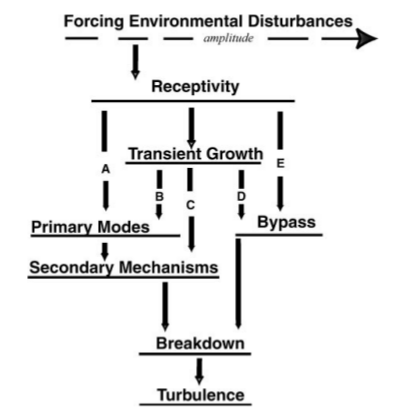
\includegraphics[scale=0.5]{path.png}
  \caption{Diffrent possible paths for transition }
  \label{fig:path}
\end{figure}

These different instabilities may occur independently or together, the
appearance of a particular type of instability depends in the Reynolds
number, wall curvature, sweep, roughness and initial conditions. The path A
is followed by weak disturbances, the initial growth of these can be
described by linear stability theory of normal modes. The growth is weak,
occurs over a long streamwise length. As the amplitude grows, 3d and
nonlinear interactions begining to occur in the form of secondary
instability. The linear stability theory can predict the transition in this
case given the free stream has weak disturbances. However, freestream can
have strong distubances which by passes the growth of linear disturbaces.
This refers to path E for which the phenomenon is yet to be explored. The
bypass refers to a transition process whose intial growth is not described
by the primary modes of Orr-Sommerfeld equation.

Transition growth occurs when two, nonorthogonal, stable modes interact,
undundergo algebraic growth, and decay exponentially. This was shown that
large amplitude can be acheived through transient growth when the boundary
layers is provided with appropriate initial condition. The spectrum of
which depends on receptivity. Generally amplitude and spectral
characteristics of the distubances inside the laminar viscous layer
strongly influence the path to be taken to turbulence.

\section{Tollmien-Schlichting (T-S) waves}

The Orr-Sommerfeld parallel flow inviscid approximation
\begin{equation}
  (U-c)\left(\phi^{\prime \prime}-\alpha^{2} \phi\right)-U^{\prime \prime}
  \phi=-\frac{i}{\alpha \operatorname{Re}}\left(\phi^{\prime \prime \prime
  \prime}-2 \alpha^{2} \phi^{\prime \prime}+\alpha^{2} \phi\right),
  \label{eq:os}
\end{equation}
have an special case when $Re \to \infty$ called Reyleigh equation given by
\begin{equation}
 (U-c)\left(\phi^{\prime \prime}-\alpha^{2} \phi\right)-U^{\prime \prime}
 \phi=0. 
  \label{eq:ra}
\end{equation}
For a boudary layer to be absolutely unstable, it must satisfy Rayleigh
criterion as a result of \Eqref{ra}. That is $D^2U = 0$, where D is the y
derivative and $Y$ is the free stream velocity profile. In other words, the
velocity profile must have an inflection point to be unstable. As the
boundary  layer profile are montonically increasing there first derivative
does not change sign, hence the boundary layers must be unconditionally
stable. However, from exprerince it is evident that boundary layers are
unstable thus inviscid approximation are not suficient to predict
instabilities in boundary layers. it can be shown using energy method that
\begin{equation}
 \frac{D E}{D t}=-\int_{V} u^{\prime} v^{\prime}\left(\frac{d U}{d
 y}\right)-\frac{1}{R} \int_{V}\left(\nabla \vec{v}^{\prime}\right)^{2}. 
  \label{eq:energy}
\end{equation}
The rightmost term is a viscous dissipation term and is stabilizing. The
leftmost term called the Reynolds stress is the primary term for instability
growth. However, in viscous flow $u^{'}$ and $v^{''}$ are non-orthogonal
due to which viscosity becomes destabilizing and is the reason for the
formation of Tollmien-Schlichting (T-S) wave.

As described by \citet{Majumdar1996}, the essential kinematic mechanism of
T-S wave can be described in terms of interaction of two "partial modes"
of the system. For system like boundary layer flow can be separated
into stable wave guides, each of which supports neutral wave in isolation,
and where wave in one waveguide may propagate in opposite direciton then in
the the other. from an energetic view point waves may have positive and negative
energy; and they are the "partial modes" in the complete system. In
boundary layer flows the inviscid modes and the viscous decaying modes are
the two partial modes. Their interaction may result in one of the following.
\begin{enumerate}
  \item if one equates the speed of the inviscid partial mode with the most
    weakly damped viscous partial mode in uniform shear, one obtains
    \Figref{6}, implies that the instability derives the interaction between the
    modes in some way.
    \begin{figure}[h!]
      \centering
      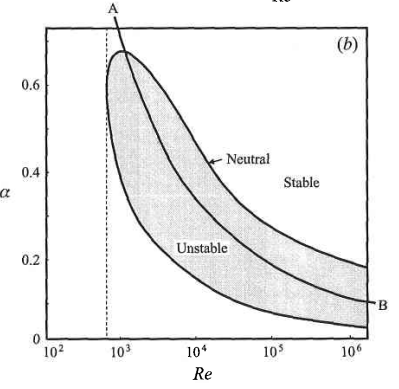
\includegraphics{6.png}
      \caption{The Stability Curve for Blasius-like profile}
      \label{fig:6}
    \end{figure}
  \item The mutual forcing must be strong enough to overcome the inherent
    damping due to viscosity.
  \item The structure of eigenfunction (\Figref{8}) for growing modes in Blasius-like
    profile resembles a superposition of an inviscid partial mode plus the
    viscous forced reponse.
    \begin{figure}[h!]
      \centering
      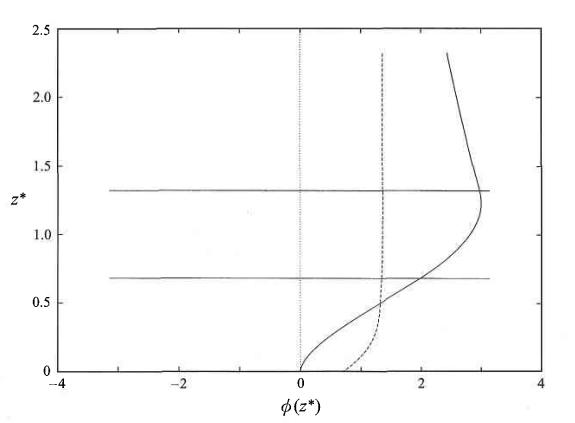
\includegraphics[scale=0.5]{8.png}
      \caption{Eigen function for Blasius-like profile}
      \label{fig:8}
    \end{figure}
\end{enumerate}
In the \Figref{tswave} showing flow ove a flat plate. From point 1 to point 2 a stable
laminar flow is established that starts from the leading edge and extends
to the point of inception of the unstable two-dimensional
Tollmien-Schlichting waves.
\begin{figure}[h!]
  \centering
  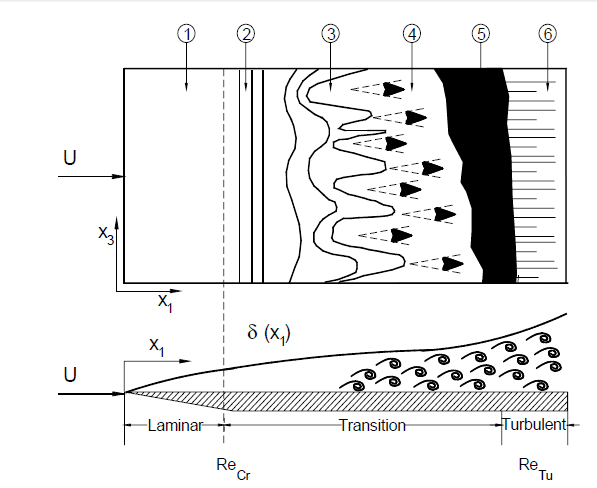
\includegraphics[scale=0.5]{xyz.png}
  \caption{The T-S wave on a flat plate}
  \label{fig:tswave}
\end{figure}

\section{Receptivity Theory}
Receptivity concerns with the generation of instability, rather their
evolution \cite{saric2002boundary}. An unsteady instability is required to
generate instabilty in
boundary layer as it is convectively unstable. The unsteady instability
can be naturally occuring or forced. Forced instability has broad wave
spectrum, thus it can be used to appropriatly excite a particular mode.
However, naturally occuring instabilities have concentrated wavenumbers,
which is different then instability wave number thus they require a
wavelength conversion process. The natural receptivity occurs where the mean
flow changes rapidly in the stream-wise direction, invalidating the
parallel flow assumption of OSE. The region where natural receptivity
occurs can be separated into two classes namely:
\begin{enumerate}
  \item Leading edge region where the boundary layer is thin
  \item Downstream region, where some local feature causes the mean flow to
    adjust on a short streamwise length scale (e.g wall humps, suction
    strip).
\end{enumerate}
\subsection{Leading-edge Receptivity Theory}
the Reynolds number is assumed to be large so that the outer problem
corresponds to the inviscid interaction of the small- amplitude freestream
disturbance with the body. The asymptotic structure for the unsteady viscous
motion in the boundary layer contains two distinct streamwise regions. The
leading edge, where $x2 \pi f /U_\infty = O(1)$, the motion satisfies the linearized,
unsteady, boundary-layer equation (LUBLE)
\begin{equation}
 u_{t}^{\prime}+U u_{x}^{\prime}+V u_{y}^{\prime}+u^{\prime}
 U_{x}+v^{\prime} U_{y}=-p_{x}^{\prime}+\left(1 / R_{L}\right) u_{y
 y}^{\prime}. 
  \label{eq:LUBLE}
\end{equation}
The LUBLE contains $u^{'} U_x$ and $V u^{'}_{y}$ which do not appear in
the OSE. Downstream from the leading edge, where $x2\pi f /U_\infty =
O(\epsilon_{LE}^{-2})$ consistent approximation leads to the classical
large-Reynolds-number, small wavenumber approximation to the OSE. The
asymptotic matching of these two regions, showed that the first
Lam-Rott asymptotic eigenfunction of the LUBLE, with coefficient $C_1$ ,
matches onto the T-S wave that becomes unstable farther downstream in the
OSE region.

The receptivity due to small-amplitude acoustic waves impinging
obliquely on the leading edge of a semi-infinite flat plate is analyzed by
separating the incident acoustic field into components parallel and
perpendicular to the plate surface. Near the leading edge, this scattered
component has a square root singularity corresponding to inviscid flow
around the sharp edge. Receptivity due to scattering of the normal component
of the incident acoustic wave is particularly important at low Mach
numbers.

the bodies of interest for practical applications gen-
erally have parabolic or elliptical leading edges and an asymmetric mean flow
owing to the presence of aerodynamic loading. In the absence of aerodynamic loading and a parallel
acoustic wave, $|C_1 |$ first rises slightly (as $S = r_{n} 2 \pi f /
U_\infty$  is increased) and then falls monotoni-
cally, to 15\% of the flat-plate value at S = 0.3. This behavior appears to be related
to the favorable pressure gradient near the nose of the parabola. For obliquely inci-
dent acoustic waves, the finite nose radius weakens the influence of leading-edge
scattering. However, as the aerodynamic
loading is increased toward its limiting value for attached flow, a strong rise in
the receptivity coefficient occurs. An attractive feature of the leading-
edge receptivity coefficient is that it is independent of frequency, f.

\subsection{Downstream region Receptivity }
Localized receptivity in the downstream is caused by the interaction of disturbances with short-scale
variations in surface geometry. An asymptotic analysis for localized receptivity,
utilizing the triple-deck structure shows that the viscous flow in the lower deck adjacent
to the wall is governed by the LUBLE. Hence, the short-scale nonparallel
mean-flow effects are again responsible for the transfer of energy from the wave-
length of the freestream disturbance to that of the instability wave.

The receptivity arises owing to nonparallel mean-flow effects, which
are expressed in terms of a perturbation series with respect to the amplitude of
the wall inhomogeneity. The OSE approach is only applicable for roughness elements of height
$h/L << R^{-5/8}_{L}$, whereas the triple-deck analysis remains valid when
$h/L = R^{-5/8}_{L}$. In the small height limit, the triple-deck equations can be solved
analytically, whereas the OSE approach requires a numerical solution.

\section{Computation Methods}
For estimatation of T-S waves modes, the spatial direct numerical simula-
tion (DNS) approach is widely applicable because it avoids many of the restrictions
that must usually be imposed in other models and is the closest to emulating exper-
iments. For example, no restrictions with respect to the form or amplitude of the
disturbances have to be imposed, because no linearizations or special assumptions
concerning the disturbances have to be made. With the spatial computational method, finite curvature can be included in the
leading-edge region. Experimentally, the most popular model geometry for receptivity has been the
flat plate with an elliptic leading edge. Thus it is reasonable that computational
models consider the same geometry. However, the curvature at the juncture between
the ellipse and the flat plate is discontinuous and provides a source of
receptivity.
Receptivity results can be expressed either in terms of (a) a leading-edge re-
ceptivity coefficient defined as the ratio of the T-S amplitude in the
leading-edge region at $x = O(U_{\infty} /2 \pi f )$ to the freestream-sound amplitude
or (b) Branch I receptivity coefficient defined as the T-S amplitude at Branch I
normalized with the freestream-sound amplitude. The appropriate receptivity
coefficient is $K_{LE}$
because it is based strictly on local properties of the leading-edge region, whereas
$K_I$ depends on the pressure gradient history from the leading edge to
Branch I.

The characteristic length scale for freestream spanwise vorticity is the
convective wavelength $U_{infty} /2 \pi f$, which is approximately three
times that of the amplified T-S wave at that frequency. A
simple model of time-periodic freestream spanwise vorticity was introduced at the
upstream computational boundary. This signal was decomposed into a symmetric
and asymmetric streamwise velocity component with respect to the stagnation
streamline. The effect of a transverse-velocity component at the leading edge
could be ascertained, as the asymmetric-velocity case had this feature, whereas
the symmetric-velocity did not.

The complete integrated picture of geometry and associated pressure
gradients (both favorable and adverse) must be included in any meaningful
evaluation of receptivity, Thus DNS analysis is favourable.

\section{Experiments For receptivity quatification}
The typical model for boundary-layer experiments is the zero-pressure-gradient
flat plate. In most cases, the flat plate is preceded by an elliptical leading-edge
attachment. The coupling between the long-wavelength acoustic disturbance
and a T-S wave occurs in four regions: the leading edge, the discontinuity in
surface curvature at the flat-plate/leading-edge junction, the presence of localized
pressure gradients, and any surface inhomogeneities such as roughness, suction
slots, or filler material used for the flat-plate/leading-edge gap.

\textbf{LARGE AMPLITUDE T-S WAVE} - When an external sound field is used as a source of disturbance
energy, the boundary-layer measurement at a particular frequency will contain
probe vibrations and a sound-wave component (Stokes layer) in addition to the
T-S wave. If these signals are of comparable amplitude, one can not extract the
T-S amplitude without some special separation technique

\textbf{REMOVABLE RECEPTIVITY SOURCE} - The simplest solution is to take advantage of the
exponential growth of the T-S wave and measure far enough downstream from
the receptivity source.

\textbf{KENDALL GAUGE} - It senses wall pressure
fluctuations at two pressure ports spaced at approximately half the T-S
wavelength. With a distribution of pressure-port pairs,
one obtains immediately the spatial behavior of the T-S wave. This method is
recommended in cases of freestream turbulence.

\textbf{COMPLEX PLANE RESOLUTION} - Taking advantage of the fact that
the acoustic wavelength is two orders of magnitude larger than the T-S wavelength,
polar plots are used to separate the long-wavelength Stokes wave from the
short-wavelength T-S wave.

\textbf{RESOLUTION OF DUCT ACOUSTICS} - The downstream traveling wave reflects in the
diffuser and returns an upstream traveling wave giving a standing wave pattern in
the test section. This is not a problem for localized receptivity sites because one
need only measure the freestream amplitude at the local position.

\textbf{PULSED-SOUND TECHNIQUE} - The technique uses pulsed sound and is
simple, effective, and lends itself to understanding the behavior of the
T-S wave.From linear theory, the maximum of the
T-S wave propagates at approximately one third of the freestream speed.
Using this fact, the traveling T-S wave can be isolated from the acoustic disturbance and associated
Stokes wave by sending bursts of sound into the test subsection

\bibliography{ref}
\end{document}

%%% Local Variables:
%%% mode: latex
%%% TeX-master: t
%%% End:
